%%%%%%%%%%%%%%%%%%%%%%%%%%%%%%%%%%%%%%%%%
% Beamer Presentation
% LaTeX Template
% Version 1.0 (10/11/12)
%
% This template has been downloaded from:
% http://www.LaTeXTemplates.com
%
% License:
% CC BY-NC-SA 3.0 (http://creativecommons.org/licenses/by-nc-sa/3.0/)
%
%%%%%%%%%%%%%%%%%%%%%%%%%%%%%%%%%%%%%%%%%

%----------------------------------------------------------------------------------------
%	PACKAGES AND THEMES
%----------------------------------------------------------------------------------------

\documentclass{beamer}

\usepackage[utf8x]{inputenc}
\usepackage[T1]{fontenc}
\usepackage{lmodern}
\usepackage[romanian]{babel}
\usepackage{amsmath}
\usepackage{listings}



\mode<presentation> {

\usetheme{Frankfurt}
\usecolortheme{dolphin}

%\setbeamertemplate{footline} % To remove the footer line in all slides uncomment this line
%\setbeamertemplate{footline}[page number] % To replace the footer line in all slides with a simple slide count uncomment this line

\setbeamertemplate{headline}{} % To remove the navigation symbols from the bottom of all slides uncomment this line
}

\usepackage{graphicx} % Allows including images
\usepackage{booktabs} % Allows the use of \toprule, \midrule and \bottomrule in tables

%----------------------------------------------------------------------------------------
%	TITLE PAGE
%----------------------------------------------------------------------------------------

\title[Parallel Graph Exploration]{Parallel Graph Exploration on Multi-Core CPU and GPU} % The short title appears at the bottom of every slide, the full title is only on the title page

\author{Vlad-Doru Ion} % Your name
\institute[UNIBUC] % Your institution as it will appear on the bottom of every slide, may be shorthand to save space
{
University of Bucharest \\ % Your institution for the title page
\medskip
}
\date{\today} % Date, can be changed to a custom date

\begin{document}

\begin{frame}
\titlepage % Print the title page as the first slide
\end{frame}

\begin{frame}
\frametitle{Overview} % Table of contents slide, comment this block out to remove it
\tableofcontents % Throughout your presentation, if you choose to use \section{} and \subsection{} commands, these will automatically be printed on this slide as an overview of your presentation
\end{frame}

%----------------------------------------------------------------------------------------
%	PRESENTATION SLIDES
%----------------------------------------------------------------------------------------

%------------------------------------------------
\section{Abstract}
%------------------------------------------------

\begin{frame}
\frametitle{Abstract}
\begin{itemize}
\item In graph-based applications, a systematic exploration of the graph such as a breadth-first search (BFS) often serves as a key component in
the processing of their massive data sets
\item We present a new method for implementing the parallel BFS algorithm on multi-core CPUs which exploits a \textbf{fundamental property of randomly shaped real-world graph instances}
\item We then propose a hybrid method which, for each level of the BFS algorithm, dynamically chooses the best implementation from: a sequential execution, two different methods of multicore
execution, and a GPU execution.
\end{itemize}

\end{frame}


%------------------------------------------------
\section{Introduction}
\begin{frame}
\frametitle{Introduction}
\begin{itemize}
\item Multi-core CPUs have become commonplace
\item There still remain, however, problems that demand fast computation but for whom efficient parallel or heterogeneous (using both CPU and GPU) implementations have yet to be identified. Graph exploration
is one important example of such problems.
\item Significant research has been
conducted to efficiently implement a parallel BFS for a wide array of computing systems
\end{itemize}

\end{frame}
%------------------------------------------------
\subsection{Existing algorithms}

\begin{frame}
\frametitle{Existing algorithms}
\begin{itemize}
\item Agarwal et al’s work which presented a state-of-the-art BFS implementation for multi-core systems

	\begin{itemize}
		\item Their implementation utilized sophisticated data structures to reduce cache coherence traffic between CPU sockets
	\end{itemize}

\item Hong et al solved the workload imbalance
issue when processing irregularly shaped graphs, which had a devastating effect on previous GPU implementations. 

	\begin{itemize}
		\item They demonstrated good performance improvement compared to
multi-core CPU implementations
	\end{itemize}

\item In this study, we build upon ideas from both previous works and incorporate them into a universal solution that utilizes both the CPU and GPU on a \textbf{heterogeneous system}.
\end{itemize}

\end{frame}
%------------------------------------------------

\begin{frame}
\subsection{Contributions of the paper}
\frametitle{Contributions of the paper}
\begin{itemize}
\item We present a BFS implementation method for multi-core
CPUs which performs better than the current state-of-theart
implementation for large graph instances, while being simpler to implement.
\item We present a hybrid method which dynamically chooses
the best execution method for each BFS-level iteration
from among: sequential execution, multi-core CPU executions,
and GPU execution.
\item We provide a fair comparison of BFS performance on
multi-core CPU and GPU, which reveals that singlesocket
high-end GPU performance can be matched by
a quad-socket high-end multi-core CPU.
\end{itemize}

\end{frame}
%------------------------------------------------

\begin{frame}
\section{Nature of Parallel BFS Algorithm on Irregular Graphs}
\frametitle{Nature of Parallel BFS Algorithm on Irregular Graphs}

Two different strategies have been proposed for parallel (and distributed) execution of BFS.

\begin{itemize}
\item The first method, known as the
\textbf{fixed-point algorithm}, continuously update the BFS level of every node, based on BFS levels of all neighboring nodes until no more updates are made
\item This method is preferred in distributed environments since it can naturally be implemented
as message passing between neighboring nodes
\item  This method potentially wastes computation,
since it processes the same edge multiple times whenever a corresponding node is updated
\end{itemize}

\end{frame}
%------------------------------------------------
\begin{frame}
\frametitle{Nature of Parallel BFS Algorithm on Irregular Graphs}
The second strategy is called \textbf{the level synchronous} BFS algorithm.

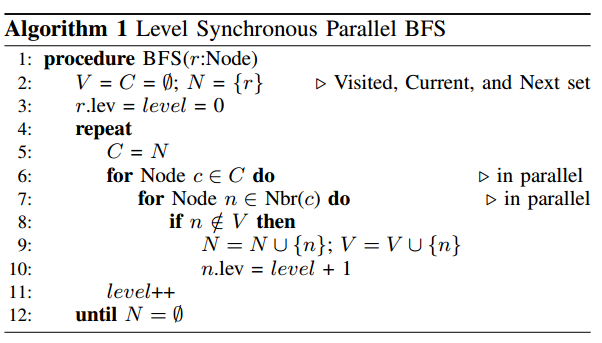
\includegraphics[scale=0.45]{algo.png}

In short, this method visits all the nodes in each BFS level
in parallel, with the parallel executions being synchronized at
the end of each level iteration.

\end{frame}
%------------------------------------------------
\begin{frame}
\subsection{Observations}
\frametitle{Observations}
\begin{itemize}
\item Nevertheless, the strategy
works quite well in practice for real-world graph instances that are irregularly shaped by nature. This is because it has been observed that the diameters of real-world graphs are small even for large graph instances, i.e. the small world
phenomenon
\item Similarly, because of the small world phenomenon the number of nodes in each BFS level cannot help but grow very rapidly,
\item Therefore the total execution time
is bounded by the traversal of the levels with a higher number of nodes, but the degree of parallelism is large in these
\end{itemize}
\end{frame}
%------------------------------------------------
\begin{frame}
\section{A new method for Multi-Core CPU}
\frametitle{A new method for Multi-Core CPU}
\begin{itemize}
\item In implementing the level synchronous parallel BFS algorithm there exists a rather direct implementation based on the presented algorithm which uses lock-protected shared queues.
\item In order to avoid significant locking overhead the following optimizations can be applied:
	\begin{itemize}
		\item Use of a bitmap to compactly represent the visited set
		\item Application of the 'test and test-and-set' operation when atomically update the bitmap.
		\item Use of local next-level queues; process node insertions into the global queue in batch.
	\end{itemize}
\item We refer to this method as the Queue-based method in the rest of this paper.
\end{itemize}
\end{frame}
%------------------------------------------------
\begin{frame}[fragile]
\frametitle{Queue-based method}
\lstset{language = C++, 
        showstringspaces=false,
        basicstyle=\ttfamily\tiny,
        keywordstyle=\color{blue},
        }
\begin{lstlisting}
BFS_Queue(G: Graph, r: Node) {
  Queue N, C, LQ[threads];
  Bitmap V;
  N.push(r); V.set(r.id);
  int level = 0; r.lev = level;
  while (N.size() > 0) {
    swap(N,C); N.clear(); // swap Curr and Next
    fork();
    for(c: C.partition(tid)) {
      for(n: c.nbrs) {
        if (!V.isSet(n.id)) {
          if (V.atomicSet(n.id)) {
            n.lev = level+1;
            LQ[tid].push(n); // local queue
            if (LQ[tid].size()==THRESHOLD){
              N.safeBulkPush(LQ[tid]);
              LQ[tid].clear();
            } 
          } 
        } 
      } 
    }
    if (LQ[tid].size() > 0) {
      N.safeBulkPush(LQ[tid]);
      LQ.clear();
    }
  join;
  level++;
  } 
}
\end{lstlisting}

\end{frame}
%------------------------------------------------
\begin{frame}
\subsection{The read-based method}
\frametitle{The read-based method}
\begin{itemize}
\item Instead of a shared queue, the
GPU implementations manage a single O(N) array.
\item Fundamentally, our approach merges and builds upon the key ideas from the previous approaches for CPU and GPU
\item In contrast to the Queue-based method,
the next-level set and the current-level set are implemented together as a single O(N) array as in the GPU implementation
\item The Read-based method provides two major advantages. First, it is completely free from queue overhead. Not only do we remove atomic instructions previously used for the queue
operations, we also save on cache and memory bandwidth. Second, the Read-based method’s memory access pattern is more sequential.
\end{itemize}

\end{frame}
%------------------------------------------------
\begin{frame}[fragile]
\frametitle{The read-based method}
\lstset{language = C++, 
        showstringspaces=false,
        basicstyle=\ttfamily\tiny,
        keywordstyle=\color{blue},
        }
\begin{lstlisting}
BFS_Read(G: Graph, r: Node) {
  Bitmap V;
  Bool fin[threads];
  V.set(r.id);
  int level = 0; r.lev = level;
  bool finished = false;
  while (!finished) {
    fork();
    fin[tid] = true;
    for(c: G.Nodes.partition(tid)) {
      if (c.lev != level) continue;
      for(n: c.nbrs) {
        if (!V.isSet(n.id)) { // test and test-and-set
          if (V.atomicSet(n.id)) {
            n.lev = level+1;
            fin[tid] = false;
          } 
        } 
      } 
    }
    join;
    finished = logicalAnd(fin, threads);
    level++;
  } 
}
\end{lstlisting}

\end{frame}
%------------------------------------------------
\begin{frame}
\frametitle{The read-based method memory access}

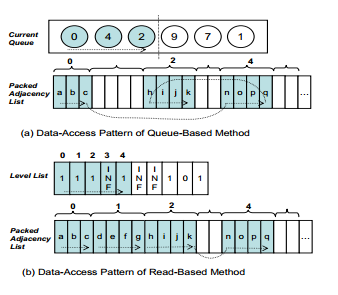
\includegraphics[scale=0.7]{memory.png}

\end{frame}
%------------------------------------------------
\begin{frame}
\frametitle{The read-based method performance}

\begin{itemize}
\item The primary disadvantage of the Read-based method is that it reads out the entire level array at every level iteration, even if only a few nodes belong to that level. However, this seldom affects the overall performance because of the following characteristics of real-world graph:
	\begin{itemize}
		\item The
diameter of the graph is small so the maximum amount of
re-read is bounded
		\item there are a few critical levels in
which the number of nodes is O(N)
		\item In addition, the total algorithm execution time
is already governed by the processing time of these critical
levels.
	\end{itemize}
\item \textit{We remind the reader that this small world property is
not merely an observation made in certain graph instances, but
rather a fundamental characteristic of randomly-shaped realworld
graphs}
\end{itemize}

\end{frame}
%------------------------------------------------
\begin{frame}
\section{Hybrid Methods}
\frametitle{Hybrid Methods}
\begin{itemize}
\item Deoarece am concluzionat că operățiile de inserare și ștergere au o complexitate timp de $\mathcal{O}(1)$ vom analiza în cele ce urmează comportamentul operației de inserare care nu este unul trivial.

\item Vom prezenta rezultatele cheie obținute în analiza complexității, deoarece demonstrația este una extrem de tehnică și nu face subiectul acestei prezentări.

\item Lucrarea inițială demonstrează că numărul mediu de iterații pentru fiecare procedură de inserare este de $\mathcal{O}(1)$, fără a ține cont de procedura de rehashing care este apelată.

\end{itemize}
\end{frame}
%------------------------------------------------
\begin{frame}
\frametitle{Analiza complexității}
\begin{itemize}

\item Se demonstrează că probabilitatea de a cauza apelarea procedurii de rehash este de $\mathcal{O}(1/n^2).$

\item În particular fiecare operație de inserție ce este efectuată în cadrul procedurii de rehashing are o probabilitate de succes de $1 - \mathcal{O}(1/n)$

\item Cum inserarea are timp $\mathcal{O}(1)$, obținem un timp mediu pentru procedura de rehashing de complexitate $\mathcal{O}(n)$. 

\item În cele din urmă combinând primul și al treilea rezultat reiese că \textbf{pentru fiecare inserție} timpul mediu pentru rehashing este de $\mathcal{O}(1/n)$, considerând șî apelarea forțată a procedurii de rehashing o dată la $r^2$ inserări.

\item În concluzie am arătat că acest algoritm prezintă o complexitate $\mathcal{O}(1)$ amortizat pentru operația de inserare.
\end{itemize}
\end{frame}
%------------------------------------------------
\begin{frame}
\section{Concluzii}
\frametitle{Concluzii}
\begin{itemize}

\item Am prezentat un algoritm cu complexitate constantă în timp pentru cazul cel mai rău.

\item Algoritmul este unul elegant și simplu de implementat, prezentând mai multe variante ale acestuia.

\item Algoritmul se comportă excelent în practică.

\end{itemize}
\end{frame}
%------------------------------------------------

\begin{frame}
\frametitle{Referințe}
\footnotesize{
\begin{thebibliography}{99} % Beamer does not support BibTeX so references must be inserted manually as below
\bibitem[cuckoo]{p1}  R. Pagh and F. F. Rodler (2002)
\newblock Cuckoo Hashing
\newblock \emph{Journal of Algorithms} 51(2004), 122 -- 144.
\bibitem[cuckoo]{p1} R.Pagh (2006)
\newblock Cuckoo Hashing for Undergraduates
\bibitem[cuckoo]{p1} Wikipedia (2014)
\newblock Cuckoo Hashing
\end{thebibliography}
}
\end{frame}

%------------------------------------------------

\begin{frame}
\Huge{\centerline{Mulțumesc}}
\end{frame}

%----------------------------------------------------------------------------------------

\end{document} 
